\documentclass{article}
\usepackage[utf8]{inputenc}
\usepackage{graphicx}
\usepackage{wrapfig}
\usepackage[super,square]{natbib}
\usepackage{tabularx}

\title{
    % \vspace{-2.5cm}
    Stewardship of Dynamical Systems
}
\author{Luke J. Pereira}
\date{}

\begin{document}

\maketitle

\section{What is water? }
To ask the reader to introspect on dynamical systems is similar to asking a fish about the water they're swimming in.\footnote
{
    This is in reference to the commencement speech delivered by the late American novelist David Foster Wallace, titled This is Water\cite{dfw}. In the speech, Wallace uses the water metaphor to bring attention to the fact that "the most obvious, ubiquitous, important realities are often the ones that are the hardest to see and talk about."
    %, with the end goal of encouraging new graduates toward disciplining their consciousness' tendencies of falling into patterns of self-centeredness, boredom, and vice.
}
It can be difficult to detach ourselves from the processes that we're actively participating in so that we can attempt to analyse them, but in fact, a deep understanding of these processes may be the only way to improve them. 

A \emph{dynamical system} can describe nearly every situation that changes or evolves over time. It is usually defined by a set of transition rules that take an initial state of a system and modifies it as time progresses. At the core of these systems, there is a sense of balance: between cause and effect, possible choices and what their branching future choices could be or cease to be, and ultimately, a balance between deterministic and stochastic behaviour. Many of us are familiar with what determinism is -- if we are 100\% sure something will happen, without any uncertainty, then it must be determined. A \emph{stochastic} process, on the other hand, produces unpredictable and random outcomes as a result of interactions between variables which all have their own likelihoods of happening. To illustrate how these seemingly very different concepts interact, we will examine a system which displays both stochastic and deterministic behaviour.

%Upon examination, we find that our mathematical models of dynamical systems have representations in nearly all natural occurring systems in reality and even in consciousness.

\section{A simple machine}
 Suppose we have a machine that follows a simple set of instructions to decide if a cell in a large paper grid will be punched in or left intact. The machine determines the state of a cell depending on the states of the nearby cells in the previous row. To make things easier to write, we can encode these elementary states with binary values $1$ and $0$, corresponding to a cell being punched in or left intact. Now we can say that if the three cells directly below a new cell are $111, 100$, or $000$, then the new cell will have state $0$, otherwise, it will be $1$.
 
\begin{wrapfigure}{r}{0.5\textwidth}
%   \vspace*{-0.4cm}
  \begin{center}
    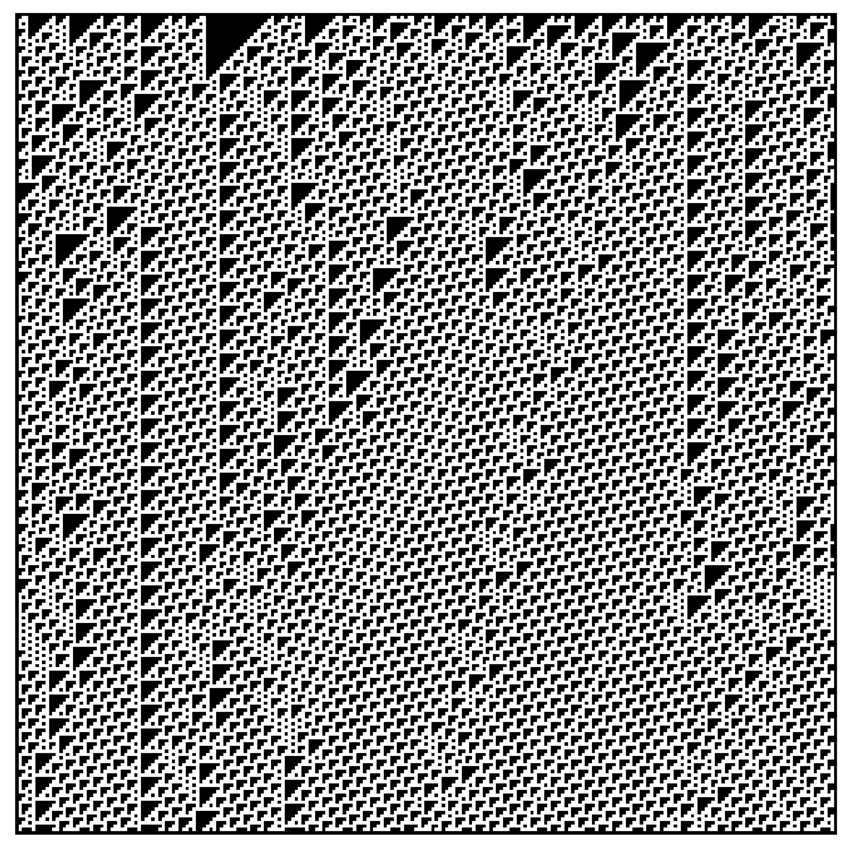
\includegraphics[width=0.5\textwidth]{class4.png}
    \caption{Magnified Rule 110}
  \end{center}
\end{wrapfigure}

From this very simple and deterministic rule, we would expect to find well-formed and predictable patterns. Instead, the machine generates results that pass the strictest mathematical tests for randomness and yet, it is not simply generating noise. The deterministic rules produce locally recognizable patterns but the global patterns are highly stochastic. The interplay between formal rules and unpredictability generates outcomes that we didn't expect and the machine appears to display its own form of creativity. If we wanted to find the state of a particular cell in a distant iteration, there would be no way for us to know what it is without running through all the computations of the cells below it. 

% The computations and the machine itself are deterministic, but the state is completely unknowable without running all the computations before it.

The machine we've described is a kind of dynamical system known as a \emph{cellular automaton}. It consists of a regular grid of cells, each of which is in one of a finite number of states. The particular system we examined is known as \emph{Rule 110} and is categorized as a class IV automaton. Members of this class of automaton all show the property we found in Rule 110, that is, their future states can not be predicted without simulating every step before it. This automaton was examined in depth by Stephen Wolfram in his 2002 book, \emph{A New Kind of Science} \cite{nks}. In it, Wolfram claims that the universe, including all the activity on our planet and in our minds, is part of a class IV automaton. For Wolfram, this claim along with the argument that no simulator could run faster than the Universe itself is sufficient grounds to argue for the existence of our free will. He suggests that even though our decisions might be predetermined because they exist in a  deterministic universe, they will still be unpredictable since the system we live in is a class IV automaton. Thus, there is no way to determine the future except to let it unfold. 


\section{An excellent servant but a terrible master}

Although not all phenomena fit perfectly into this cellular-automata conception of the world, it's undeniable that dynamical systems can be found all around us and have serious impacts on our daily lives and our well-being. Despite all of this, we still have little insight into many of their inner workings, like their transition rules or possible states. It's likely that, because we are overwhelmed by the complexity and unpredictability of the systems, we assume the rules which define them are equally complex so we avoid trying to understand or safeguard them. Moreover, because of the growing complexity of the systems around and within us, it's more important now than ever before in the past for us to attempt to steward these systems so they do not run amok, which could result in depletion of our natural resources, geopolitical conflicts, and even mass mental health issues. It has only recently become crucial for future generations to master these systems which were automatic and unconscious to us in previous generations.

There is a Buddhist saying, ``The mind makes an excellent servant but a terrible master''. It expresses an understanding that the mind requires guidance developed from self-discipline and spiritual training, otherwise, it has a tendency of falling into patterns of self-centred thoughts, boredom, and can form habits of vice. The saying brings to light the balance between our conscious deterministic thoughts and our unconscious stochastic mental patterns. This sentiment regarding the mind can also be expressed about many other dynamical systems of our modern society that are also prone to fall into patterns with destructive consequences. Unrestrained capitalist and consumerist global markets tend to result in environmental and wealth distribution issues, a lack of family planning policies can result in overpopulation, not providing young people with mental health guidance and training can result in increased depression and suicide rates, etc. It is important for us to acknowledge that even though issues may exist on very complex global scales, they are likely restrained to a simple set of rules that dictate their interactions and future states. From this perspective, it is entirely possible and perhaps necessary for individuals to make an effort to introduce safeguards in the form of intelligent and creatively designed rules and regulations that can help push our global society towards a more favourable and sustainable future. 


\begin{thebibliography}{9}
\bibitem{dfw}
Foster., Wallace, David (2009). This is water: some thoughts, delivered on a significant occasion about living a compassionate life. Kenyon College. (1st ed.). New York: Little, Brown. ISBN 0316068225.

\bibitem{nks}
Wolfram, Stephen (2002). A New Kind of Science. Champaign, IL. Wolfram Media. 1579550088.

\end{thebibliography}
\end{document}
